%% LyX 2.4.2.1 created this file.  For more info, see https://www.lyx.org/.
%% Do not edit unless you really know what you are doing.
\documentclass[twoside]{article}
\usepackage[LGR,T1]{fontenc}
\usepackage[utf8]{inputenc}
\pagestyle{headings}
\usepackage{color}
\definecolor{note_fontcolor}{rgb}{0.800781, 0.800781, 0.800781}
\usepackage{url}
\usepackage{amsmath}
\usepackage{amssymb}
\usepackage[authoryear]{natbib}

\makeatletter

%%%%%%%%%%%%%%%%%%%%%%%%%%%%%% LyX specific LaTeX commands.

% Repeats stuff from master preamble
% I think that's OK...
\usepackage{tikz}
\usetikzlibrary{arrows,automata,positioning,arrows.meta}


\DeclareRobustCommand{\greektext}{%
  \fontencoding{LGR}\selectfont\def\encodingdefault{LGR}}
\DeclareRobustCommand{\textgreek}[1]{\leavevmode{\greektext #1}}

%% Because html converters don't know tabularnewline
\providecommand{\tabularnewline}{\\}
%% The greyedout annotation environment
\newenvironment{lyxgreyedout}
{\normalfont\normalsize\textcolor{note_fontcolor}\bgroup\ignorespaces}
{\ignorespacesafterend\egroup}

\makeatother

\usepackage[english]{babel}
\begin{document}
To evaluate our proposed survey designs, we must first construct our
ICKMR model for walrus. We encode our knowledge about walrus biology
and life history to (\textit{i}) build a model of walrus population
dynamics, including the breeding cycle, and (\textit{ii}) formulate
kinship probabilities between pairs of samples. The population dynamics
model incorporates demographic parameters that will need to be estimated:
survival rates, adult abundance in some reference year, trend, and
so on. The kinship probabilities depend on the population dynamics.
Given a real dataset, we would estimate the parameters by maximizing
the log-likelihood that combines the kinship probabilities with the
actual outcomes of all pairwise comparisons. For design purposes,
though, we instead use a computational shortcut to predict the precision
of the estimates that would be expected under different sampling designs.
Although it is not strictly necessary to simulate any data in this
process, we did use simulations to check that our CKMR model was appropriately
formulated. This section describes our population dynamics model,
kinship probability formula, design calculations, and simulation setup.

\subsection{Biological considerations}

Adult males are inaccessible to this study given seasonal sex-segregation
and the geographical coverage of sampling effort (see Section \ref{sec:Introduction}).
They also form leks and compete for breeding access to females, so
it is plausible that adult males might also exhibit persistent individual
variability in breeding success, which would considerably complicate
the interpretation of paternal half-sibling kinship data (see Discussion).
Therefore, we restrict attention to female-only dynamics, and consider
only three types of kinship: Mother-Offspring Pair (MOP), Cross-cohort
maternal Half-Sibling Pair (XmHSP), and Self Pair (SP), i.e. recapture
of an individual. Our samples comprise juvenile and adult females,
plus juvenile males; the problems are with modelling males as parents,
but we can safely use sampled juvenile males as potential offspring
of females and as potential maternal half-siblings of other (female
or male) samples. We do not expect females to vary much in terms of
individual fecundity.

We assume that age estimates will be available for all samples, based
on epigenetic data (CITE). Visual classification is only accurate
over the first couple of years of life (CITE), which could be problematic
for CKMR. Our model is structured to allow for errors in estimated
age (with standard deviation assumed known i.e., after calibration
of epigenetic against known-age samples), though the results here
assume that there are no errors; see Discussion.

\subsubsection{Stage-structured quasi-equilibrium dynamics}

For our female-only population dynamics model, we opted for a stage-structured
(juvenile/adult), rather than fully-age-structured approach. We did
this because (\textit{i}) most female adults are expected to have
similar reproductive capacity and chance of survival, regardless of
age; and (\textit{ii}) stage-structured models are simpler to code
for CKMR and require fewer parameters (the addition of IMR data makes
things less simple). Stage-structured results should be quite adequate
for design purposes; the fundamental role of total (non-age-specific)
adult abundance and survival is very similar to fully-age-structured
models.

We used two stages: juveniles aged 1–5, and adults aged 6+ (the first
age at which an accompanying calf is common) at sampling. We did not
consider calves (age 0), to avoid complications around mother-calf
sampling. We assume constant survival within each stage ($\phi_{\text{A}}$
and $\phi_{\text{J}}$), and that offspring survival from age 1 onwards
is independent of its mother's survival, whether or not the offspring
has weaned yet. We assume that adult female abundance is stable, increasing,
or decreasing exponentially over the period covered by the population
dynamics (2000–2028; the lower limit of $y_{0}=$2000 is set because
there were fairly drastic changes in the population prior to that).
We have
\begin{align}
N_{y,\text{A}} & =N_{y_{0},\text{A}}e^{r(y-y_{0})}\label{popdyn}
\end{align}
where $N_{y,\text{A}}$ is the abundance of adult females in year
$y$, and $e^{r}$ is the rate of population increase.

Age composition within stage does not matter for MOP and XmHSP probabilities,
but is relevant for SPs. For that purpose, we assume that age composition
over the period is adequately described by the stable-age or ``quasi-equilibrium\textquotedbl{}
distribution consistent with survival $\phi_{\text{A}}$ and rate-of-increase
$e^{r}$. As shown in e.g., \citet{keyfitz2005applied} Chapter 5,
this is  $N_{y,a}\propto N_{y,\text{A}}\phi_{\text{A}}^{a}e^{-ra}$.

\subsubsection{The breeding cycle\label{subsec:The-breeding-cycle}}

We use a Markov model to describe the walrus breeding cycle. We assume
three breeding states: (S1) pregnant; (S2) with young-of-the-year
(YOTY) calf; or (S3) non-breeding, i.e., neither of the above. The
Markov property assumes that next year's state depends only on this
year's. From state S1 (pregnant), next year's state must be S2 (with
YOTY calf). From state S2, a female may next year either return to
state S1 (become pregnant again), with probability $\psi_{2}$, or
move to state S3 (neither pregnant nor with calf) with probability
$1-\psi_{2}$. From state S3, she will either move to state S1 (become
pregnant) with probability $\psi_{3}$, or remain in state S3 with
probability $1-\psi_{3}$. Due to long gestation times (\textasciitilde 14
months), walrus cannot give birth to calves in two consecutive years
(CITE). We also allow $\psi_{2}\neq\psi_{3}$ as they are unlikely
to give birth to calves every second year (CITE). This is shown in
Figure~\ref{fig:Breeding-cycle}. Survival is assumed to be independent
of breeding state. Females enter state S3 (i.e., reach sexual maturity)
on reaching age 4, and therefore can become pregnant at age 5 and
give birth at age 6. Depending on the values of $\psi_{2}$ and $\psi_{3}$,
this leads to a ramping-up in effective fecundity (i.e., probability
of being in state S2) over the first few years of adult life. Both
$\psi_{2}$ and $\psi_{3}$ are estimated from the data. We do not
use any data on whether females were with/without calf when sampled,
so the estimates of $\psi_{2}$ and $\psi_{3}$ are ultimately reliant
on the distribution of birth-gaps between maternal half-sibling pairs.

\begin{figure}
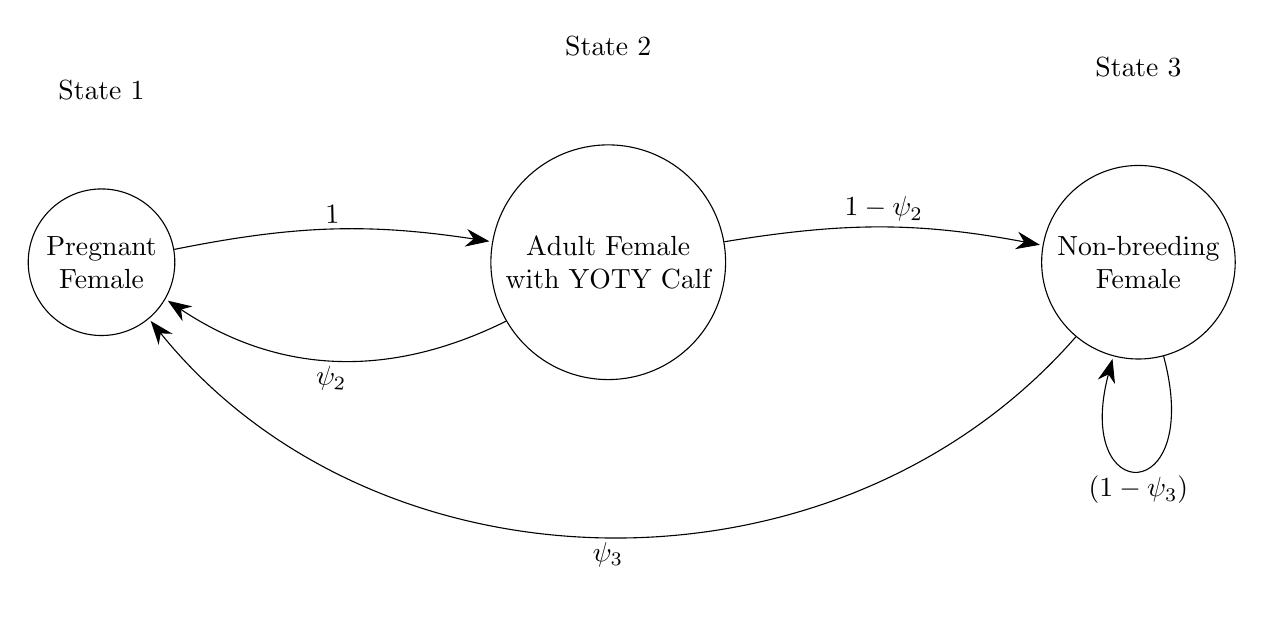
\begin{tikzpicture}[
    shorten > = 1pt,
node distance = 1cm and 4cm,
    el/.style = {inner sep=2pt, align=left, sloped}
                    ]

\node (q0) [state, align = center]             {Pregnant \\ Female};
\node (q1) [state,right=of q0, align = center] {Adult Female \\with YOTY Calf};
\node (q2) [state,right=of q1, align = center] {Non-breeding\\ Female};

\path[arrows=-{Stealth[length=3mm]}] 
    (q0)  edge [bend left=10]  node[el,above]  {$1$}         (q1)
    (q1)  edge [bend left=10]  node[el,above]  {$1-\psi_2$}         (q2)
    (q2)  edge [bend left=50]  node[el,below]  {$\psi_3$}         (q0)
    (q1)  edge [bend left=30]  node[el, below] {$\psi_2$}  (q0)

    ;

\draw[->,>= {Stealth[length=3mm]}]      (q2)  edge [loop below] node[el,below] {$(1-\psi_3)$}   (q2);

\node (e1)  [above=of q0] {State 1};
\node  (e2) [above=of q1] {State 2};
\node (e3) [above=of q2] {State 3};
\end{tikzpicture}

\caption{Directed cyclic graph showing the breeding cycle for walrus as represented
in our Markov model. Nodes in the graph show the states (pregnant,
with young-of-the-year (YOTY) calf, or non-breeding) and edges give
the probabilities of transition between those states. Walrus reach
sexual maturity at age 4, so females enter the graph at node non-breeding.
\label{fig:Breeding-cycle}}
\end{figure}

We will later use two quantities, which are derived from the breeding
cycle. First, we need to calculate the (average) proportion of adult
females in S2, $\bar{\beta}_{2}$. Let $\Psi$ be the (3$\times$3)
transition matrix implied by Figure~\ref{fig:Breeding-cycle}. Taking
the the eigendecomposition of $\Psi$, we can extract the second element
of the eigenvector with the largest eigenvalue to obtain $\bar{\beta}_{2}$.
We can then define fecundity as a function of age
\begin{gather}
F\left(a\right)\triangleq\frac{\mathbb{P}\left[B\left(a\right)=2\right]}{\bar{\beta}_{2}},\label{eq:fec-def}
\end{gather}
so that immature animals have fecundity 0, and an average adult has
fecundity 1.

\subsubsection{Formulating kinship probabilities}

We now need to formulate the demographic probabilities that two samples
have a given kinship, using the ERRO principle. We write the kinship
for individuals $i$ and $j$ as $K_{ij}$, which in our case may
be MOP, XmHSP, SP, or UP. In the case of MOPs and XmHSPs, we take
care to use only one sample from each individual (so ``sample''
and ``individual'' are interchangeable terms), whereas for SPs we
need to consider multiple samples from one individual (in which case,
``sample'' and ``individual'' have different meanings).

Throughout we use the following notation: for individual \emph{$i$},
sampled at age $a_{i}$ in year $y_{i}$ with birth year $b_{i}\triangleq y_{i}-a_{i}$.
As noted above, we only consider female abundance, so throughout $N$
refers to females only. When female abundance is considered for a
given year ($y$) and development stage ($d=\text{A}$ or $\text{J}$,
for adult or juvenile, respectively), it is written with two arguments,
$N_{y,d}$. We define the binary variable $L$ to indicate lethality
of sampling ($L_{i}=1$ indicating lethal sampling for individual
$i$). We use $\mathbb{I}()$ as an indicator function, giving 1 when
the condition inside the brackets is true, else 0. Kinship probabilities
are functions of demographic parameters such as $\phi_{\text{A}}$and
$N_{y_{0},\text{A}}$; we use $\boldsymbol{\theta}$ as shorthand
for this set of parameters, which become explicit in later iterations
of the formulae.

\subsubsection{Mother-offspring pairs (MOPs)}

Suppose we are about to compare a potential mother \emph{i}, to a
potential offspring \emph{j}. We restrict attention to comparisons
that satisfy the following:
\begin{itemize}
\item \emph{$i$} is female (though \emph{$j$} need not be);
\item $a_{j}\geqslant1$ (no calf samples are used);
\item $b_{j}\geqslant2000$ (population dynamics starts at year 2000).
\end{itemize}
We can now distinguish two cases: $y_{i}<b_{j}$ and $y_{i}\geqslant b_{j}$.

For $y_{i}<b_{j}$, individual \emph{i} still has to survive several
years in order to be individual \emph{j}'s mother (note that \emph{i}
may be immature when sampled, but mature by the time of \emph{j}'s
birth). In this case $i$'s sampling \textit{must} be non-lethal ($L_{i}=0$).
The MOP probability is
\[
\mathbb{P}\left[K_{ij}=\text{MOP}\vert a_{i},y_{i},b_{j},L_{i}=0,\boldsymbol{\theta}\right]=\frac{R_{i}(b_{j}\vert y_{i},a_{i})}{R^{+}(b_{j})}.
\]
where $R_{i}(b_{j}\vert y_{i},a_{i})$ is the expected reproductive
output (ERO) of individual $i$ in year $b_{j}$ given $i$ is age
$a_{i}$ in year $y_{i}$. $R^{+}(b_{j})$ is the total reproductive
output (TRO) of the whole population in year $b_{j}$. ERO and TRO
are in units of \textquotedbl number of calves\textquotedbl{} here
(though generally their units are arbitrary but matching). TRO is
the total number of adult females in the population when $j$ is born,
$N_{b_{j}\text{A}}$, multiplied by the proportion of females with
calves (breeding state S2), $\bar{\beta_{2}}$: $R^{+}(b_{j})=\bar{\beta_{2}}N_{b_{j},\text{A}}$.

There are two components to $i$'s ERO: first, she has to survive;
second, she has to be calving (breeding state 2) in $b_{j}$:
\[
R_{i}\left(b_{j}\vert y_{i},a_{i}\right)=\Phi\left(y_{i}-b_{j},a_{i}\right)\mathbb{P}\left[B\left(a_{i}+b_{j}-y_{i}\right)=2\right],
\]
where $\Phi\left(\Delta t,a\right)$ gives the probability of survival
for $\Delta t$ years, starting from age $a$ (product of annual juvenile
and adult survival probabilities). $B\left(a\right)$ is an individual's
breeding state in year $a$, which here is individual \emph{$i$}'s
age at $b_{j}$ ($a_{i}+b_{j}-y_{i}$, assuming she survives).

Then, using our definition of fecun\ref{eq:MOP-future}dity at age,
\eqref{eq:fec-def}, we have
\begin{gather}
\mathbb{P}\left[K_{ij}=\text{MOP}\vert a_{i},y_{i},b_{j},L_{i}=0,y_{i}<b_{j},\boldsymbol{\theta}\right]=\frac{\Phi\left(y_{i}-b_{j},a_{i}\right)F\left(a_{i}+b_{j}-y_{i}\right)}{N_{b_{j},\text{A}}}.\label{eq:MOP-future}
\end{gather}

If \emph{$i$} is sampled after $j$'s birth ($b_{j}<y_{i}$). We
then know \emph{$i$} was alive (or not born yet), so there are no
lethality nor survival terms to worry about, but she may not have
been mature. Letting $F\left(a\leqslant0\right)=0$ (walruses cannot
breed before birth),
\begin{gather}
\mathbb{P}\left[K_{ij}=\text{MOP}\vert a_{i},y_{i},b_{j},b_{j}<y_{i},\boldsymbol{\theta}\right]=\frac{F\left(a_{i}-y_{i}-b_{j}\right)}{N_{b_{j},\text{A}}}.\label{eq:MOP-past}
\end{gather}


\subsubsection{Maternal half-sibling pairs (XmHSPs)}

We now find the probabilities of cross-cohort (X), maternal (m), half-sibling
pairs (HSP): XmHSPs. We want to compare individual \emph{$k$} to
individual \emph{$l$}, to check whether they have the same mother.
We restrict attention to comparisons that satisfy the following criteria:
\begin{itemize}
\item $b_{l}>b_{k}$ (avoiding double-counting);
\item $b_{k}\neq b_{l}$ (walrus give birth to a single offspring at a time);
\item $b_{k}\geqslant2000$ (population dynamics starts at 2000).
\end{itemize}
We know that $k$ definitely had a mother, whom we shall call $m$.
What is the probability that $l$'s mother was also $m$, given what
we know about $m$? The latter is that \textit{\emph{ }}\emph{$m$}
was alive, mature, and in breeding state S2 at $k$'s birth, andalso
\emph{$m$} survived at least one more year after\emph{ }$k$'s birth,
otherwise \emph{$k$} would not have lived long enough to be sampled.
In order for \emph{$m$} to be $l$'s mother, three more things have
to happen:
\begin{enumerate}
\item $m$ survives until $b_{l}$;
\item $m$ is in breeding state S2 in $b_{l}$;
\item amongst all the females that are alive and in the right breeding state
in year $b_{l}$, $m$ is the one who happens to be $l$'s mother.
\end{enumerate}
Let $\Phi\left(\Delta t\right)$ be the adult probability of survival
for $\Delta t$ years from \textquotedbl now\textquotedbl{} and recall
$\Psi$ is the breeding cycle transition matrix. The probability 3-vector
of an animal being in each state (S1, S2, S3) at time $t$ is $p^{\left[t\right]}$.
The probability vector at time $t+1$ is then $p^{\left[t+1\right]}=\Psi p^{\left[t\right]}$.
Now define $p^{\left[0\right]}=\left(0,1,0\right)^{\top}$which is
the probability vector of \emph{$m$}'s breeding state at $k$'s birth
(certain state 2), and recall $\bar{\beta}_{2}$ is the proportion
of adult females in breeding state S2. Then

\begin{gather}
\mathbb{P}\left[K_{k\ell}=\text{XmHSP}|b_{k},b_{\ell},\theta\right]\nonumber \\
=\mathbb{P}\left[K_{km}=\text{MOP}|B_{m}\left(b_{k}\right)=\text{S2},m\text{ alive at }b_{k}+1,b_{\ell},\theta\right]\nonumber \\
=\frac{\Phi\left(b_{l}-b_{k}-1\right)\left[\Psi^{b_{l}-b_{k}}p^{\left[0\right]}\right]_{2}}{N_{b_{l},\text{A}}\bar{\beta}_{2}}\label{eq:xmhsp}
\end{gather}

where $\left[\right]_{2}$ gives the second element of the vector,
i.e. the probability that \textit{m} (given she was alive) was again
in breeding state S2 at \textit{l}'s birth.

HSPs are just one of several ``second-order'' kin-pairs that are
practically indistinguishable genetically, hence cannot be identified
directly and unambiguously. Fortunately, HSPs are demographically
the most common when the birth-gap is short. When the birth-gap approaches
twice the age-of-maturity, though, GGPs (Grandparent-Grandchild Pair)
are more common. We deal with this by restricting the range of birth
gaps used in the model to those where GGPs are very rare (e.g., below
twice the age at maturity).

\subsubsection{Self-recaptures (SPs)\label{subsec:selfPs}}

Our stage-structured model keeps the population dynamics simple, but
we do have to make extra assumptions about sampling selectivity to
include the IMR data. Here, we assume that selectivity varies only
by stage (adult/juvenile), not by age within stage. We only consider
female samples for self-recapture, since juvenile males are prone
to \textquotedbl permanent emigration\textquotedbl{} (CITE) as well
as true mortality, so do not yield readily-interpretable inferences.

To compute stage-structured self-recapture probabilities, we condition
on the age of the first sample but \emph{not} explicitly on the age
of the second sample; instead we condition on the second sample's
developmental stage at sampling ($d_{2}$). If the first sample would
have reached the right developmental stage (otherwise, the two cannot
be the same animal), then we assume it is equally likely to be \emph{any}
of the females in that developmental stage at that year (i.e., sampling
is unselective within developmental stage) and thus the chance it
is the same as the second sample is the reciprocal of the developmental
stage abundance. We must also include survival for the intervening
years. The self-recapture kinship probability between samples 1 and
2 is (where $y_{1}<y_{2}$):

\begin{gather}
\mathbb{P}\left[K_{12}=\text{SP}\vert a_{1},y_{1},d_{2},y_{2},L_{1}=0,\boldsymbol{\theta}\right]=\frac{\mathbb{I}\left[d\left(a_{1}+\left(y_{2}-y_{1}\right)\right)=d_{2}\right]\Phi\left(y_{2}-y_{1},a_{1}\right)}{N_{y_{2},d_{2}}},\label{eq:self-staged}
\end{gather}
where $d\left(a\right)$ is the function that maps age to developmental
stage, with $d\left(a<6\right)=\text{"juvenile"}$ and $d\left(a\geqslant6\right)=\text{"adult"}$.
We also condition on the first sample being non-lethal (since we have
a second sample). To obtain $N_{y_{2},d_{2}}$, adult abundance is
part of the population dynamics model, but some more work is required
to deduce juvenile abundance. Assuming stable age composition, we
show in Appendix \ref{sec:Deriv-Njy} that for walrus:

\[
N_{y,\text{J}}=N_{y,\text{A}}\frac{\rho-\phi_{\text{A}}}{\rho-\phi_{\text{J}}}\left(\left(\frac{\rho}{\phi_{\text{J}}}\right)^{5}-1\right),
\]
where $\rho=e^{r}$ is the relative annual population increase/decrease.

A purely-age-structured version of \eqref{eq:self-staged} would need
to explicitly keep track of numbers-at-age, not just adult abundance
(as would the other kin types). The quasi-equilibrium assumption might
allow us to do this, but that assumption directly constrains relative
abundances-at-age. Thus, for example, the age 10 samples would then
provide direct estimates of the abundance of age 30 samples. In practice,
a fully age-structured CKMR formulation for walrus will need something
more sophisticated and time-varying than a quasi-equilibrium age distribution,
and therefore additional parameters to estimate. We therefore opted
for a stage- rather than age-structured SP model in the hope that
the overall statistical information content about total abundance
is reasonably realistic compared to what we might get from a more
complicated population dynamics model.

\subsection{Simulations}

We developed an individual-based simulation with the life history
and population dynamics of Pacific walrus to test our ICKMR model.
The simulation was modified from the R package \texttt{fishSim} by
Shane Baylis (\url{https://github.com/SMBaylis/fishSim}). The simulation
is stochastic and operates on an annual basis. Individuals are tracked
through the use of unique identifiers so that kinship pairs can be
identified in simulated samples. We initialized the simulation in
1950 with a population of 250,000 animals. These individuals are considered
``founders'' and do not have mothers or fathers. The age and sex
structure of the initial population is determined by the survival
rates used in the simulation (Table~\ref{tab:demo-pars}), which
were based on rates reported in \citet{taylor_demography_2018}. Individuals
that are at or beyond the age of first reproduction mate randomly
and males can potentially father more than one calf. Females reproduction
follows Section~\ref{subsec:The-breeding-cycle}. Females that are
in state 2 of the breeding cycle give birth to a single offspring
with 1:1 sex ratio. There is no systematic age-effect on female reproductive
dynamics, except that they are guaranteed not-pregnant in the year
immediately prior to maturity (Section~\ref{subsec:The-breeding-cycle}),
which slightly lowers effective fecundity for the first few years
of adulthood until the Markov chain reaches equilibrium. We did not
include senescence in our CKMR model, but we do include it in our
simulations. Parameters in Table~\ref{tab:demo-pars} were adjusted
to maintain the desired population rate of increase ($r$).

In sampling years, captures are simulated according to either historical
or planned future sample sizes. Females are available to be sampled
at any age, while only calf and juvenile males are available for sampling.
For simulated captures between 2014 and 2017, we used the realized
sample sizes by age or age class as the basis for simulation. For
simulated captures between 2023 and 2027, we used the target number
of samples per age class as the basis for simulation. After sampling,
some individuals die (according to age and/or sex specific mortality
rates, Table \ref{tab:demo-pars}). If a female with a young-of-the-year
calf dies, her calf also dies. Individuals automatically die if they
reach the maximum age. Living individuals then have their age incremented.

The female breeding cycle is as described in Section \ref{subsec:The-breeding-cycle}.
Although we assume in the simulation that all pregnancies result in
live births, this rate is aliased with the nominal calf-survival probability,
since only samples from age 1 onwards are considered; only the product
(nominal pregnancy success rate $\times$ nominal calf survival) affects
the simulated samples, not the two constituent parameters. Males and
females < 4 (or > the age of last reproduction; ALR) are exempt from
this cycle. The simulation then proceeds to the following year.

All simulations had a starting population size of 250,000 and were
run from 1950 to 2030. 

\begin{table}
\caption{Demographic parameters for simulation under four scenarios (D0, D1,
D2, and D3)\label{tab:demo-pars}}

\begin{tabular}{ccccc}
 & \multicolumn{4}{c}{Demographic Scenario}\tabularnewline
\cline{2-5}
 & D0 & D1 & D2 & D3\tabularnewline
Parameter & NULL & Stable & Decreasing & Increasing\tabularnewline
\hline 
Maximum age (AMAX) & 37 & 37 & 37 & 37\tabularnewline
Age at first reproduction for females (AFR) & 6 & 6 & 6 & 6\tabularnewline
Age of last reproduction for females (ALR) & 37 & 29 & 29 & 29\tabularnewline
Age of first reproduction for males & 15 & 15 & 15 & 15\tabularnewline
Young-of-the-year (Age 0 calf) survival & 0.7 & 0.7 & 0.66 & 0.7\tabularnewline
Juvenile survival (Ages 1 to 5) & 0.9 & 0.9 & 0.85 & 0.9\tabularnewline
Reproductive adult female survival (Ages 6 to ALR) & 0.9622 & 0.99 & 0.985 & 0.99\tabularnewline
Non-reproductive adult female survival (Ages ALR to AMAX) & NA & 0.55 & 0.5 & 0.55\tabularnewline
Probability of breeding at 2-yr interval (\emph{\textgreek{ψ}}\textsubscript{2}) & 0.1 & 0.1 & 0.1 & 0.1\tabularnewline
Probability of breeding at 3-yr+ interval (\emph{\textgreek{ψ}}\textsubscript{3}) & 0.5 & 0.5 & 0.5 & 0.5\tabularnewline
Resulting rate of increase (\emph{r}) & 0 & 0 & -0.02 & +0.01\tabularnewline
\end{tabular}
\end{table}
\begin{table}
\caption{Sampling scenarios\label{tab:Sampling-scenarios}}

\begin{tabular}{cccccccc}
 &  & \multicolumn{6}{c}{Effort per Year}\tabularnewline
\cline{3-8}
Sampling Scenario & Description & 2023 & 2024 & 2025 & 2026 & 2027 & 2028\tabularnewline
\hline 
S0 & NULL: 100\% effort 2023-20287 & 1 & 1 & 1 & 1 & 1 & 0\tabularnewline
S1 & Reality + 100\% effort 2025-2026 & 1 & 0 & 1 & 1 & 0 & 0\tabularnewline
S2 & Reality + 100\% effort 2025-2027 & 1 & 0 & 1 & 1 & 1 & 0\tabularnewline
S3 & Reality + 100\% effort 2025-2028 & 1 & 0 & 1 & 1 & 1 & 1\tabularnewline
S4 & Reality + 75\% effort 2025-2026 & 1 & 0 & 0.75 & 0.75 & 0 & 0\tabularnewline
S5 & Reality + 75\% effort through 2027 & 1 & 0 & 0.75 & 0.75 & 0.75 & 0\tabularnewline
S6 & Reality + 75\% effort through 2028 & 1 & 0 & 0.75 & 0.75 & 0.75 & 0.75\tabularnewline
S7 & 100\% effort 2023-2025 & 1 & 1 & 1 & 0 & 0 & 0\tabularnewline
\end{tabular}
\end{table}


\subsection{Model checking}

To evaluate agreement between the simulation and CKMR model, we generated
50 replicate simulated datasets with demographic parameters under
a null scenario as in Table \ref{tab:demo-pars} demographic scenario
D0 and simulated historical and future sampling according to realized
or target sample sizes by age class, with effort per year from 2023
as in sampling scenario S0 in Table \ref{tab:Sampling-scenarios}).
We checked each of the simulated datasets against the CKMR model for
observed and expected numbers of kin pairs in different categories
(MOPs, XmHSPs, and SPs), observed versus expected gaps between half-sibling
pairs, and the log-likelihood derivatives at the true parameter values.
See Section \ref{sec:Model-checking}for details.

\subsection{Survey design}

We were interested in evaluating the performance of CKMR under different
demographic and sampling scenarios. The demographic scenarios were
a stable population (D1), a slightly decreasing population (D2) and
a slightly increasing population (D3). Demographic parameters for
these simulated scenarios are shown in Table \ref{tab:demo-pars}.
For these simulations, we simulated historical sampling according
to realized sample sizes by age and sex, and future sampling by target
sample sizes by age class. We simulated scenarios with (L2) and without
(L1) the collection of 100 lethal samples per year in sampling years.%
\begin{lyxgreyedout}
This is where we-all might wanna consider investigatin wotif a LOT
more lethal ones; 100 is too small to help.%
\end{lyxgreyedout}
{} We also simulated various reductions in sampling effort, either by
reducing the number of sampling years or by reducing the amount of
sampling effort within years (S1-S7; Table \ref{tab:Sampling-scenarios}).
With three demographic scenarios, two lethality scenarios, and seven
sampling scenarios, this resulted in a total of 42 simulated datasets
from which to evaluate survey design.

\subsection{Design calculations}

CKMR sampling designs can often be evaluated by calculation alone.
These calculations are based on adapting standard methods used to
find the statistical information from the (pseudo-)likelihood (i.e.,
its derivatives) and enumerating the pairwise comparisons that would
be required based on covariate combinations (which are few, given
we have a relatively small range of covariates; e.g., age, year of
sample, etc).

Let $w_{ijk}$ be the kinship outcome for samples $i$ and $j$ and
target kinship $k$: $w_{ijk}=1$ if their actual kinship $K_{ij}=k$,
or 0 if $K_{ij}\neq k$; and let $w=\left\{ w_{ijk};\forall i,j,k\right\} $
(in practice, some ``impossible'' comparisons are excluded; e.g.,
second-order kin born a long time apart). Define $p_{ijk}\left(\boldsymbol{\theta}\right)=\mathbb{P}\left[K_{ij}=k\vert z_{i},z_{j},\boldsymbol{\theta}\right]$
to be the kinship probability for samples $i$ and $j$, parameter
values $\boldsymbol{\theta}$ and covariates $z_{i}$ and $z_{j}$
(computed from e.g., \eqref{eq:MOP-future}). In each case the probability
that $w_{ijk}=1$ is on the order of the reciprocal of adult abundance
(very small), and is well approximated by a Poisson distribution with
mean $p_{ijk}\left(\boldsymbol{\theta}\right)$. The pseudo-log-likelihood
is:

\[
\Lambda\left(\boldsymbol{\theta};\mathbf{w}\right)=C+\sum_{i<j;k\in\mathcal{K}}\left\{ -p_{ijk}\left(\boldsymbol{\theta}\right)+w_{ijk}\log_{e}p_{ijk}\left(\boldsymbol{\theta}\right)\right\} ,
\]
where $C$ is a constant and $\mathcal{K}$ are the kinship relationships
being considered.

We use $H\left(\boldsymbol{\theta}_{0}\right)$=$d^{2}\Lambda\left(\boldsymbol{\theta}_{0};\mathbf{W}\right)/d\boldsymbol{\theta}^{2}$
(the expected Hessian) over datasets $\mathbf{W}$ at true parameter
values $\boldsymbol{\theta}_{0}$. As $\Lambda$ is a sum of individual
comparison terms, so is $H\left(\boldsymbol{\theta}_{0}\right)=\sum_{i<j;k\in\mathcal{K}}h_{ijk}\left(\boldsymbol{\theta}_{0}\right)$,
where

\[
h_{ijk}\left(\boldsymbol{\theta}_{0}\right)=4\boldsymbol{\Delta}_{ijk}\left(\boldsymbol{\theta}_{0}\right)\boldsymbol{\Delta}_{ijk}\left(\boldsymbol{\theta}_{0}\right)^{\top}\qquad\text{where }\boldsymbol{\Delta}_{ijk}\left(\boldsymbol{\theta}\right)=\frac{d\sqrt{p_{ijk}\left(\boldsymbol{\theta}\right)}}{d\boldsymbol{\theta}}.
\]
$\boldsymbol{\Delta}_{ijk}\left(\boldsymbol{\theta}\right)$ can be
obtained efficiently for all $(i,j,k)$ by numerical differentiation
of the probabilities calculated by the ICKMR model, using some reasonable
guess about $\boldsymbol{\theta}_{0}$. %
\begin{lyxgreyedout}
using squared 1st derivatives is the Fisher information? Can we call
this the pseudo-Fisher information? Oh, sorry, I always get confused
by which one is the formal definition (2nd D, or 1st D \textasciicircum 2).
The thing is that under ``sparse sampling'', the two will be the
same here anyway... let's wing it ;)%
\end{lyxgreyedout}

We can now exploit the small range of possible covariates and group
across all pairs with identical covariate values. Let $m(\mathbf{z})$
denote the number of samples with covariate combination $\mathbf{z}$;
the number of comparisons between two samples is $m\left(\mathbf{z}_{1}\right)m\left(\mathbf{z}_{2}\right)$.
The grouped version of the expected Hessian can be written as 

\begin{gather}
H\left(m_{\mathcal{Z}};\boldsymbol{\theta}_{0}\right)=\sum_{\mathbf{z}_{1}<\mathbf{z}_{2}\in\mathcal{Z};k\in\mathcal{K}}m\left(\mathbf{z}_{1}\right)m\left(\mathbf{z}_{2}\right)h\left(\mathbf{z}_{1},\mathbf{z}_{2},k\right),\label{eq:H-grouped}
\end{gather}
where $h\left(\mathbf{z}_{1},\mathbf{z}_{2},k\right)$ is the single-comparison
expected Hessian for two samples with covariates $\mathbf{z}_{1}$
and $\mathbf{z}_{2}$ respectively%
\begin{lyxgreyedout}
\footnote{The ordering ``$z_{1}<z_{2}$'' is arbitrary, included just to avoid
double-counting. Sometimes it makes sense to also do comparisons with
$z_{1}=z_{2}$, in which case an extra factor of 1/2 is required.}%
\end{lyxgreyedout}
. The set $\mathcal{Z}$ comprises all possible combinations of covariates,
and $m_{\mathcal{Z}}$ is the corresponding breakdown of total sample
size by covariate combinations (e.g., year, age, sex). We can then
invert \eqref{eq:H-grouped} to give the average predicted variance
$V\left(m_{\mathcal{Z}};\theta_{0}\right)$ of a parameter estimate.
Uncertainty from any function of the parameters, $g\left(\boldsymbol{\theta}\right)$,
can then be approximated by the delta method:
\[
\mathbb{V}\left[g\left(\boldsymbol{\theta}\right);m_{\mathcal{Z}},\boldsymbol{\theta}_{0}\right]\approx\left[\left.\frac{dg\left(\boldsymbol{\theta}\right)}{d\boldsymbol{\theta}}\right\vert _{\boldsymbol{\theta}_{0}}\right]V\left(m_{\mathcal{Z}},\boldsymbol{\theta}_{0}\right)\left[\left.\frac{dg\left(\boldsymbol{\theta}\right)}{d\boldsymbol{\theta}}\right\vert _{\boldsymbol{\theta}_{0}}\right]^{\top}.
\]

While a ``design'' must, by definition, include some specification
of sample sizes, it may not specify the full breakdown of samples
into specific $\mathbf{z}$-categories. For example, the plan might
be to sample 1000 adult walruses per year, but the age composition
cannot be controlled directly. However, we still need to know $m_{\mathcal{Z}}$,
so some extra assumptions and calculations might be required. For
example, our population-dynamics model does not explicitly represent
the adult age composition within the population, let alone within
the samples; probabilities like \eqref{eq:MOP-past} are \emph{conditioned}
on sample age, but make no prediction about how many samples of each
age there will be. It would be possible to calculate expected sample
sizes based on quasi-stable age compositions and unselective sampling
assumptions (assumptions that are implicit for the self-recapture
probability \eqref{eq:self-staged}), but somewhat laborious. Since
we are simulating sampled datasets in any case, the simulated sample
composition can be used directly for $m_{\mathcal{Z}}$.

The proposed walrus sample size (about 15,000 in total) is large relative
to adult female abundance (\textasciitilde 70,000; effectively more
because of turnover during the years modelled), so \textasciitilde 10\%
of samples are self/kin-recaptures. This means that a comparable proportion
of pairwise comparisons have predictable outcomes based on the results
of other comparisons, breaking independence. The ``sparse sampling''
assumption of \citet{bravington_close-kin_2016} is therefore not
strictly justified, so the variance might be slightly over- or under-estimatedrelative
to our calculations here; the direction is not obvious. %
\begin{lyxgreyedout}
I am changing my thinking about this; it's highly not obvious...%
\end{lyxgreyedout}
{} (there is no effect on point estimates). Appendix \ref{appendix:Adjustments-for-non-sparse}
details some effective sample size adjustments to our calculations
in order to account for the non-independence of the pairwise comparisons.
\end{document}
